\section{Slučajevi upotrebe}

\subsection{Pristupanje mreži}

\begin{figure}[h!]
		\centerline{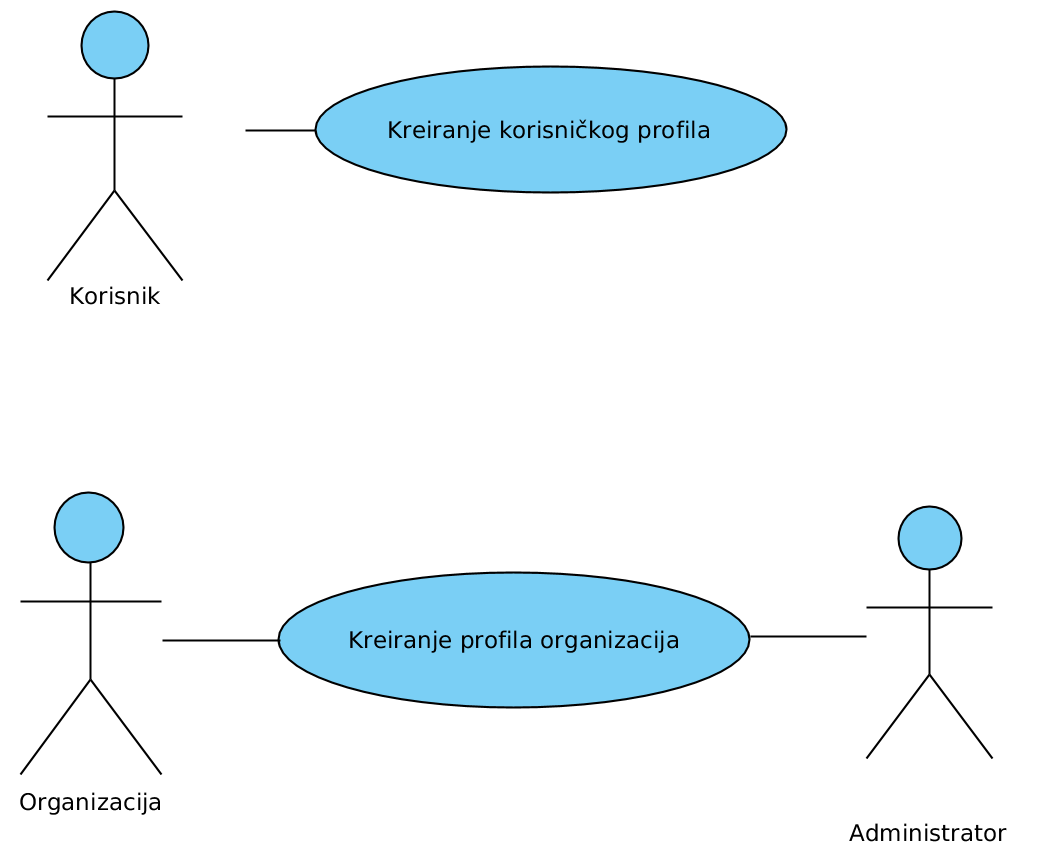
\includegraphics[width=\textwidth]{slike/pridruzivanje.png}}
		\captionof{figure}{Dijagram slučaja upotrebe za pridruživanje mreži}
\end{figure}

\subsubsection{Kreiranje korisničkog profila}
\begin{itemize}
	\item Kratak opis - Korisnik se registruje tako što popunjava formu svojim ličnim podacima. Nakon validacije unetih podataka korisnik prelazi na sledeći korak. Kako bi upotpunio kreiranje profila bira oblasti interesovanja na osnovu kojih će mu objave biti filtrirane.
	\item Učesnici - neregistrovan korisnik
	\item Preduslovi - korisnik ima pristup internetu
	\item Postuslovi - korisniku je kreiran nalog
	\item Glavni tok
	\begin{enumerate}
		\item Korisnik odlazi na stranicu za registrovanje novih korisnika
		\item Korisnik unosi lične podatke i klikne na dugme "Sledeći korak"
		\item Vrši se validacija podataka
		\item Na sledećoj strani korisnik bira oblasti interesovanja prema kojim će mu se prikazivati objave (bira iz padajuće liste sa opcijom pretraživanja)
		\item Korisnik klikne na dugme "Završi registraciju"
		\item Sistem privremeno čuva unete podatke
		\item Korisniku je stigao aktivacioni e-mail sa linkom za potvrdu registracije
		\item Korisnik otvara mail i klikne na link za potvrdu registracije
		\item Sistem aktivira nalog
		\item Korisnik dobija obaveštenje da je nalog kreiran
	\end{enumerate}
	\item Alternativni tokovi
	\begin{itemize}
		\item[3.a] Nevalidna prijava - sistem ukazuje korisniku na kom polju forme podaci nisu korektno uneti. Slučaj upotrebe se nastavlja na koraku 2.
		\item[7.a] Korisnik nije potvrdio registraciju u odredjenom vremenskom intervalu - link za potvrdu je istekao. Slučaj upotrebe se završava
	\end{itemize}
\end{itemize}

\subsubsection{Kreiranje profila organizacija}
\begin{itemize}
	\item Kratak opis - Organizacije pristupaju mreži tako što popunjavaju formu odgovarajućim podacima. Tu formu proverava administrator nakon čega odobrava profil. Time organizacija postaje ravnopravan član mreže.
	\item Učesnici - organizacija i administrator
	\item Preduslovi
	\begin{itemize}
		\item Organizacija je validno pravno lice koje može pristupiti mreži 
		\item Organizacija ima pristup internetu
	\end{itemize}
	\item Postuslovi - organizaciji je kreiran nalog
	\item Glavni tok
	\begin{enumerate}
		\item Organizacija odlazi na stranicu za registrovanje organizacija
		\item Organizacija unosi podatke i klikne na dugme "Završi unos podataka"
		\item Sistem proverava unete podatke
		\item Sistem obaveštava organizaciju o uspešnosti inicijalne provere podataka i daje mogućnost korigovanja unetih podataka.
		\item Organizacija klikne na dugme "Završi registraciju"
		\item Uneti podaci se šalju administratoru na pregled
		\item Administrator odobrava pristup organizacije socijalnoj mreži i šalje e-mail za potvrdu naloga
		\item Organizacija potvrđuje nalog korišćenjem linka poslatog e-mailom
		\item Sistem aktivira nalog
		\item Organizacija dobija obaveštenje da je nalog kreiran
	\end{enumerate}
	\item Alternativni tokovi
	\begin{itemize}
		\item[3.a] Uneti podaci nisu ispravni - sistem ukazuje koji podaci nisu adekvatni. Slučaj upotrebe se nastavlja na koraku 2.
		\item[7.a] Organizacija nije validan korisnik mreže. Administrator šalje e-mail kojim obaveštava organizaciju da je njihov zahtev za pristup mreži odbijen. Slučaj upotrebe se završava.
		\item[8.a] Link za potvrdu naloga je istekao. Slučaj upotrebe se završava.
	\end{itemize}
\end{itemize}

\subsection{Ažuriranje profila}
\begin{itemize}
	\item Kratak opis - Korisnik može menjati svoje lične podatke ili oblasti interesovanja
	\item Učesnici - korisnik, organizacija
	\item Preduslovi - korisnik je registrovan (organizacija se pridružila mreži) i ulogovan
	\item Postuslovi - izmenjeni su željeni podaci
	\item Glavni tok
	\begin{enumerate}
		\item Korisnik (organizacija) odlazi na stranicu za ažuriranje podataka klikom na opciju "Izmeni profil"
		\item Sistem prikazuje formu koja sadrži podatke koji se mogu menjati
		\item Korisnik (organizacija) pravi željene izmene
		\item Klikom na opciju "Sačuvaj" potvrdjuje izmene
		\item Sistem ažurira napravljene izmene
	\end{enumerate}
\end{itemize}

\subsection{Kreiranje korisničkih grupa}
\begin{itemize}
	\item Kratak opis - Korisnik ili organizacija mogu kreirati grupu koja je jedinstveno određena nazivom. Sadržaj grupe su objave koje odgovaraju temi grupe.
	\item Učesnici - Korisnik ili organizacija
	\item Preduslovi - Korisnik ili ogranizacija je registrovana na mrežu
	\item Postuslovi - Grupa je kreirana i može se pronaći na socijalnoj mreži 
	\item Glavni tok
    \begin{enumerate}
		\item Korisnik klikne na dugme "Kreiraj grupu" nakon čega mu se prikazuju polja za unos naziva grupe i kratkog opisa.
		\item Korisnik bira da li će sadržaj grupe biti vidljiv ili skriven korisnicima mreže koji nisu članovi grupe.
		\item Poziva korisnike ili organizacije da se učlane u grupu.
    \end{enumerate}
\end{itemize}


\subsection{Deljenje sadržaja}
\begin{itemize}
	\item Kratak opis - Korisnici mreže mogu kreirati objave koje će biti prikazane odabranoj publici. Odabir publike vrši sam kreator pažljivim odabirom oblasti na koje se objava odnosi. Takođe, mogu se targetirati i studenti određenih fakulteta.
	\item Učesnici - korisnici mreže
	\item Preduslovi - učesnici su registrovani
	\item Postuslovi - kreirana objava vidljiva je na profilu korisnika i na početnim stranama targetiranih korisnika
	\item Glavni tok
    	\begin{enumerate}
		\item Korisnik klikne na dugme "Kreiraj novu objavu" nakon čega mu se prikazuju polja za unos
		\item Bira tip objave: obaveštenje, pitanje, tutorijal ili ponuda
		\item Popunjava polja karakteristična za tip objave (podtok)
		\item Unosi tekst objave gde može i da označi druge korisnike
	    	\item Bira oblasti na koje se objava odnosi
	    	\item Može da izabere opciju za vidljivost objave
	    	\item Može da izabere odredjene fakultete ukoliko postoji povezanost sa sadržajem
		\item Nakon klika na dugme "Objavi", sistem validira objavu 
	    	\item Ukoliko je objava validna, sistem obrađuje podatke, upisuje u bazu i objava je kreirana
    	\end{enumerate}
	\item Podtok - popunjavanje polja karakterističnih za tip objave
    	\begin{itemize}
        	\item Ukoliko je izabran "tutorijal"
            	\begin{enumerate}
	         	\item Kreator mora da učita fajl
	         	\item Mora da izabere folder ili kreira novi radi organizacije tutorijala
	         	\item Može da označi saradnike na tutorijalu
            	\end{enumerate}
         	\item Ukoliko je izabrana "ponuda"
            	\begin{enumerate}
            		\item Kreator mora da navede tip ponude (npr rad na projektu, ponuda za posao/praksu, držanje časova, i slično)
            	\end{enumerate}    
	 \end{itemize}
	 \item Alternativni tok
	 \begin{enumerate} 
	 	\item Objava nije validna, kreiranje objave je stopirano
	 \end{enumerate}
\end{itemize}
\begin{figure}[h!]
		\centerline{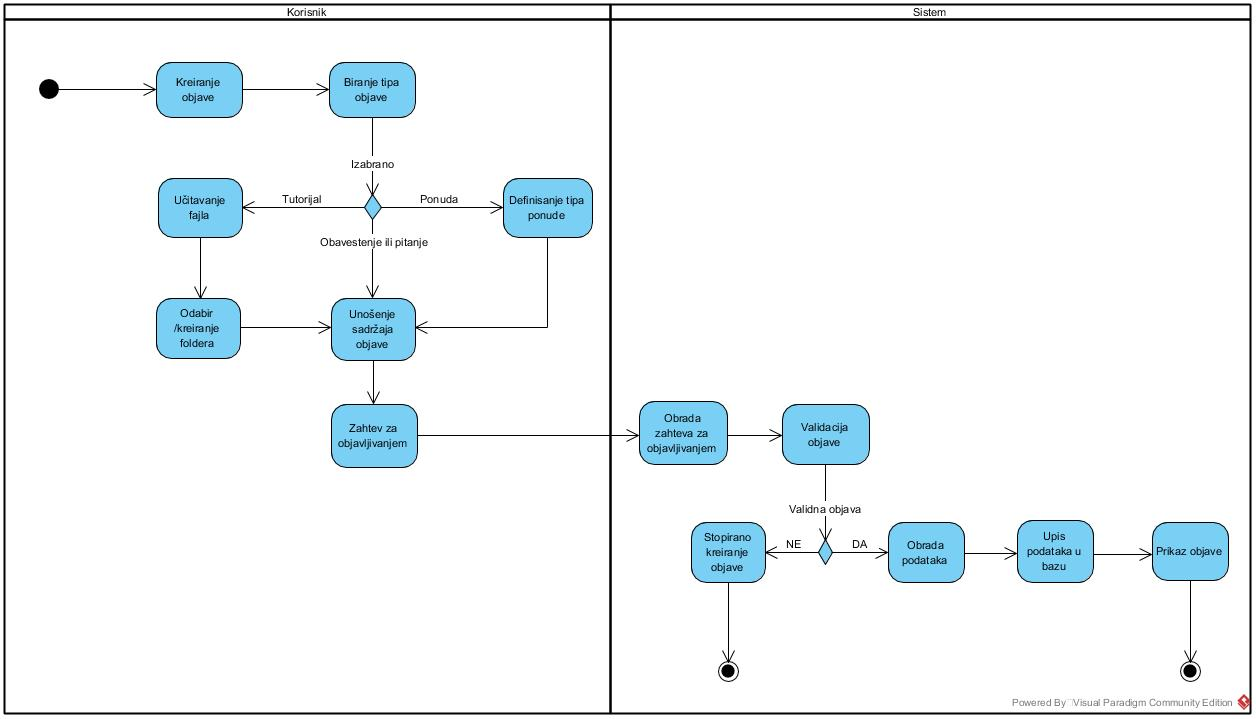
\includegraphics[width=\textwidth]{slike/deljenje_sadrzaja.jpg}}
		\captionof{figure}{Dijagram aktivnosti za deljenje sadržaja}
\end{figure}

\subsection{Pretraživanje}
\subsubsection{Pretraživanje i pregled profila/grupa}
\begin{itemize}
	\item Kratak opis - Korisnici i organizacije mogu vršiti pretragu i pregled profila drugih korisnika (organizacija), kao i pretragu i pregled sadržaja grupa.
	\item Učesnici - Korisnici, organizacije
	\item Preduslovi - Korisnik (organizacija) - registrovani
	\item Postuslovi - Prikazani su svi profili/grupe koji zadovoljavaju kriterijum pretrage, omogućen je pregled njihovog sadržaja
	\item Glavni tok
	\begin{enumerate}
		\item Korisnik (organizacija) unosi u polje za pretragu karakter '@' a zatim i filter pretrage i klikne na dugme "Pretraga"
		\item Prikazuju se svi profili/grupe koji u svom nazivu imaju uneti filter pretrage
		\item Korisnik (organizacija) može da klikne na naziv profila/grupe i pregleda njihov sadržaj
	\end{enumerate}
	\item Alternativni tok
	\begin{enumerate}
		\item Nije pronadjen traženi profil/grupa
		\item Sve dok korisnik (organizacija) želi da vrši pretragu, poništava filter pretrage i unosi novi
	\end{enumerate}
\end{itemize}


\subsubsection{Pretraživanje objava}
\begin{itemize}
	\item Kratak opis - Korisnici i organizacije mogu vršiti pretragu objava koje u svom sadržaju imaju unete filtere pretrage, odnosno unete tagove. Filteri i tagovi se mogu kombinovati. Omogućava se lakše pronalaženje sadržaja koji interesuje korisnike mreže.
	\item Učesnici - Korisnici, organizacije
	\item Preduslovi - Korisnik (organizacija) - registrovani
	\item Postuslovi - Prikazane su sve objave koje zadovoljavaju kriterijum pretrage 
	\item Glavni tok
	\begin{enumerate}
		\item Korisnik (organizacija) unosi u polje za pretragu filter pretrage (ili vise njih), odnosno za svaki tag unosi karakter '\#' a zatim i naziv taga i klikne na dugme "Pretraga"
		\item Prikazuju se sve objave koje u svom sadržaju imaju unete filtere/tagove
		\item Korisnik (organizacija) može da klikne na objavu i pregleda njen sadržaj
	\end{enumerate}
	\item Alternativni tok
	\begin{enumerate}
		\item Nije pronadjena tražena objava
		\item Sve dok korisnik (organizacija) želi da vrši pretragu, poništava filtere/tagove pretrage i unosi nove 
	\end{enumerate}
\end{itemize}

\subsection{Kontrolisanje sistema}
\subsubsection{Kontrolisanje sadržaja}
\begin{itemize}
	\item Kratak opis - Administrator vrši kontrolu objavljenog sadržaja, kako ne bi došlo do deljenja neodgovarajućeg sadržaja. 
	\item Učesnici - Administrator
	\item Preduslovi - Korisnik (organizacija) - registrovani
	\item Postuslovi - Sadržaj koji je objavljen na mreži od strane korisnika (organizacija) je u skladu sa politikom socijalne mreze
	\item Glavni tok
	\begin{enumerate}
		\item Administrator dobija informaciju o podeljenom sadržaju koji nije u skladu sa politikom mreže
		\item Izvršava proveru objave
		\item Administrator uklanja objavu ukoliko je neodgovarajućeg sadržaja
		\item Izvršava kontrolu profila korisnika (organizacije) koji je podelio objavu (opisano u narednom slučaju upotrebe)
	\end{enumerate}
\end{itemize}


\subsubsection{Kontrolisanje profila}
\begin{itemize}
	\item Kratak opis - Administrator vrši kontrolu nad profilima korisnika (organizacija) kako ne bi došlo do zloupotrebe mreže. 
	\item Učesnici - Administrator, korisnik, organizacija
	\item Preduslovi - Korisnik (organizacija) - registrovani
	\item Postuslovi -Podaci na profilima korisnika (organizacija) su ispravni i u skladu sa pravilima mreže
	\item Glavni tok
	\begin{enumerate}
		\item Administrator dobija informaciju o sumnjivim podacima na profilu korisnika (organizacije)
		\item Izvršava proveru podataka
		\item Ukoliko se ispostavi da su podaci neodgovarajući, administrator obaveštava korisnika (organizaciju) o tome
		\item Ukoliko korisnik (organizacija) ne izmeni neodgovarajuće podatke na svom profilu, administrator uklanja profil sa mreže
	\end{enumerate}
\end{itemize}


\subsection{Komentarisanje objava}
\begin{itemize}
	\item Kratak opis - Korisnik postavlja komentar na bilo koju vrstu objave (svoju ili objavu drugog korisnika). 
	\item Učesnici - Korisnik
	\item Preduslovi - Korisnik je registovan na mrežu
	\item Postuslovi - Komentar je uspešno postavljen i vidljiv ostalim korisnicima mreže.
	\item Glavni tok
	\begin{enumerate}
		\item Korisnik piše komentar na objavi.
		\item Nakon završetka pisanja komentara, korisnik koristi dugme "Pošalji komentar". 
		\item Komentar je objavljen i vidljiv ostalim korisnicima mreže.
	\end{enumerate}
	\item Alternativni tokovi
    \begin{itemize}
		\item[3.a] Korisnik je uneo prazan komentar. Slučaj upotrebe se završava.
	\end{itemize}
\end{itemize}

\subsection{Ocenjivanje}
\begin{itemize}
	\item Kratak opis - Korisnik ocenjuje objavu ili komentar bilo kog korisnika mreže, pri čemu korisnicima nije dozvoljeno ocenjivanje sopstvenih objava ili komentara. Ocenjivanje se vrši uvećavanjem ili umanjenjem ukupne ocene za jedan.
	\item Učesnici - Korisnik
	\item Preduslovi - Korisnik je registovan na mrežu
	\item Postuslovi - Ocena je prihvaćenja i konačna ocena objave ili komentara je ažurirana.
	\item Glavni tok
	\begin{enumerate}
		\item Korisnik postavlja pozitivnu ili negativnu ocenu na komentar ili objavu koristeći odgovarajuće dugme za to.
		\item Nova ocena je uspešno uračunata u ukupnu ocenu odgovarajuće objave ili komentara.
	\end{enumerate}
	\item Alternativni tokovi
    \begin{itemize}
		\item[1.a] Korisnik je već izvršio ocenjivanje na dotičnom sadržaju. Slučaj upotrebe se završava.
	\end{itemize}
\end{itemize}

\subsection{Komunikacija}
\begin{itemize}
\item Kratak opis - Korisnici ili organizacije koriste ugrađene funkcionalnosti sistema za međusobnu interakciju. Komunikacija se ostvaruje slanjem poruke ili odgovaranjem na primljenu poruku.
\item Učesnici - Korisnik, organizacija
\item Preduslovi 
    \begin{itemize}
	\item Korisnik je član mreže
	\item Organizacija je član mreže
	\end{itemize}
\item Postuslovi - Poruka je uspešno poslata i vidljiva primaocu iste.
\item Glavni tok
	\begin{enumerate}
		\item Korisnik ili organizacija pristupa profilu željenog korespodenta.
		\item Pritiskom na dugme "Poruka", otvara se prozor. 
		\item Unosi se željeni tekst u otvorenom prozoru. 
		\item Pritiskom na dugme "Pošalji", šalje se poruka korespodentu.
		\item Primalac poruke dobija obaveštenje o novoj poruci.
		\item Primalac može odgovoriti na dobijenu poruku unošenjem teksta na odgovarajuće mesto.
		\item Pritiskom na dugme "Odgovori", šalje se odgovor.
		\item Koraci 6, 7 i 8 se ponavljaju sve dok se ne završi komunikacija.
	\end{enumerate}
\item Alternativni tokovi
    \begin{itemize}
		\item[4.a] Korisnik je uneo praznu poruku. Poruka se ne šalje, slučaj upotrebe se nastavlja od koraka 3.
		\item[7.a] Primalac je uneo praznu poruku. Poruka se ne šalje, slučaj upotrebe se nastavlja od koraka 6.
	\end{itemize}
\end{itemize}
\begin{figure}[h!]
		\centerline{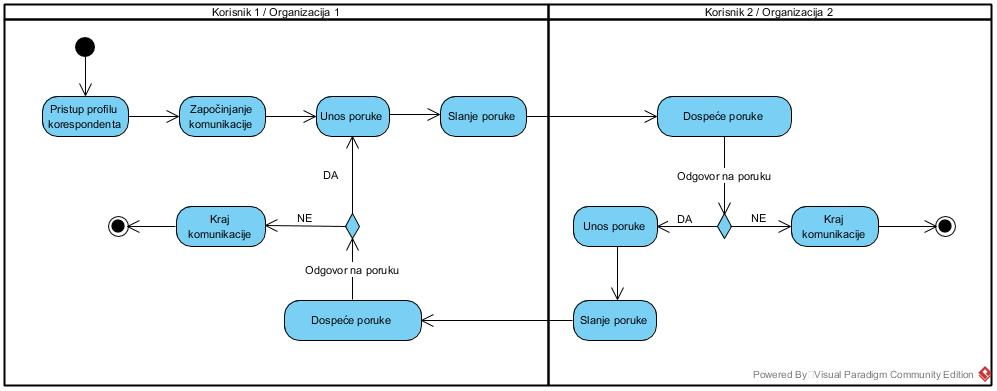
\includegraphics[width=\textwidth]{slike/komunikacija.jpg}}
		\captionof{figure}{Dijagram aktivnosti za komunikaciju}
\end{figure}

\subsection{Prijava}
\subsubsection{Prijavljivanje na korisnički profil}
\begin{itemize}
	\item Kratak opis - Korisnik (ili organizacija) se prijavljije na profil koji je prethodno kreirao.
	\item Učesnici - korisnik ili organizacija
	\item Preduslovi - korisnik ima pristup internetu i ima napravljen profil na socijalnoj mreži.
	\item Postuslovi - korisnik se uspešno prijavio na svog profil
	\item Glavni tok
		\begin{enumerate}
			\item Korisnik pristupa veb stranici socijalne mreže
			\item U polje za unos e-maila unosi svoj mail
			\item U polje za unos lozinke unosi svoju lozinku
			\item Korisnik pritiska dugme "Prijavi se" 
		\end{enumerate}
	\item Alternativni tokovi
	    \begin{itemize}
	        \item[4.a] Neuspešna prijava - korisnik je uneo neispravnu lozinku. Slučaj upotrebe se nastavlja na koraku 3. ili prelazi na slučaj upotrebe "zaboravljena lozinka"
	    \end{itemize}
\end{itemize}
\subsubsection{Zaboravljena lozinka}
\begin{itemize}
    \item Kratak opis - Proces koji korisnik (organizacija) obavlja u slučaju da je zaboravio lozinku
    \item Učesnici - korisnik, organizacija
    \item Preduslovi - korisnik ima pristup internetu
    \item Postuslovi - korisnik je uspešno promenio lozinku
    \item Glavni tok
        \begin{enumerate}
	        \item Korisnik(organizacija) bira opciju "Zaboravili ste lozinku"
	        \item Otvara se nova stranica na kojoj bira način na koji će promeniti lozinku (putem email-a ili broja telefona)
	        \item Bira opciju "Nastavi" i otvara mu se nova stranica
	        \item Korisniku (organizaciji) stiže kod za promenu lozinke na email (telefon)
	        \item Unosi kod u polje na stranici i bira opciju "Nastavi"
	        \item Unosi novu šifru dva puta
	        \item Bira opciju "Promeni lozinku"
	        \item Dobija informaciju da je lozinka uspešno promenjena
        \end{enumerate}
    \item Alternativni tokovi
        \begin{itemize}
            \item[4.a] Korisnik nije uneo kod u odredjenom vremenskom intervalu. Slučaj upotrebe se završava.
            \item[7.a] Korisnik nije uneo oba puta istu lozinku. Slučaj upotrebe se nastavlja na koraku 6.
            
        \end{itemize}
\end{itemize}
\subsection{Odjavljivanje sa korisničkog profila}
\begin{itemize}
	\item Kratak opis - Korisnik (ili organizacija) se odjavljuje sa profila na koji se prethodno prijavio.
	\item Učesnici - korisnik ili organizacija
	\item Preduslovi - korisnik ima pristup internetu i prijavljen je na svoj profil
	\item Postuslovi - korisnik se uspešno odjavio sa svog profila, na koji se može opet prijaviti u bilo kom trenutku.
	\item Glavni tok
		\begin{enumerate}
			\item Korisnik pristupa stranici svog profila
			\item Korisnik pritiska dugme "Odjavi se"
		\end{enumerate}
\end{itemize}
\subsection{Deaktiviranje profila}
\begin{itemize}
	\item Kratak opis - Korisnik (ili organizacija) deaktivira profil koji koristi na mreži.
	\item Učesnici - korisnik ili organizacija
	\item Preduslovi - korisnik ima pristup internetu i prijavljen je na svoj profil
	\item Postuslovi - korisnik je uspešno deaktivirao svoj profil, koji se ne može više koristiti za pristup mreži.
	\item Glavni tok
		\begin{enumerate}
			\item Korisnik pristupa stranici za deaktiviranje profila
			\item Korisnik unosi svoju lozinku u odgovarajuće polje
			\item Pritiskom na dugme "Deaktiviraj profil", korisnik dobija upozorenje da će njegov profil i podaci koji su vezani za isti biti izgubljeni.
			\item Pritiskom na dugme "OK", profil se briše iz baze podataka.
		\end{enumerate}
	\item Alternativni tokovi
		\begin{itemize}
			\item[3.a] Korisnik je uneo neispravnu lozinku, slučaj upotrebe se nastavlja od koraka 2.
			\item[4.a] Pritiskom na dugme "Poništi", korisnik se vraća na početnu stranu i njegov profil nije deaktiviran. Slučaj upotrebe se završava.
		\end{itemize}
\end{itemize}




